\documentclass{article}
\usepackage[T2A]{fontenc}
\usepackage[utf8]{inputenc}
\usepackage[russian]{babel}
\usepackage{amssymb,amsmath,amsthm}
\usepackage{systeme,mathtools}
\usepackage{lipsum}
\usepackage{relsize}
\newcommand\md{\ }
\usepackage[normalem]{ulem}
\usepackage{pdfpages}

\begin{document}
\selectlanguage{russian}

\includepdf[pages=-]{ok.pdf}
\section{Введение}
SimInTech является средой для создания математических моделей
любых систем, уравнение динамики которых можно представить в виде
входо-выходных соотношений (представление DataFlow). 

\section{Постановка задачи}

Для демонстрации моделирования с использованием конечных автоматов используется модель управления водонагревательным котлом. 
Если температура ниже заданной, то контроллер обеспечивает включение нагревателя на время не более 20 секунд, с выдержкой между включениями 40, а также индикацию состояния с помощью включения и выключения лампочки индикации.
При включенном нагревателе мощность нагрева постоянна и нагревает 1 литр воды на 1 градус за секунду.
При выключенном нагревателе потери постоянны и таковы, что охлаждают 1 литр воды на 0,1 градуса за секунду.
Количество воды - 25 литров.

В качестве входных воздействии в регулятор задаются:
1. Заданное значение температуры, которую необходимо обеспечить;
2. Текущее значение температуры, полученной от датчика температуры.

\section{Описание модели в терминах конечных автоматов}

Автомат имеет два состояния: «включен» и «выключен». Переход между состояниями: из состояния «выключен» в состояние «включен» осуществляется в случае совпадения двух условий: контроллер находится в состоянии «выключен» более 40 с и температура с датчика ниже заданной уставки.

Переход из состояния «включен» в состояние «выключен» осуществляется в двух случаях:
1. Нагрев осуществлялся в течении 20 секунд;
2. Температура с датчика достигла заданной уставки.

В начальный момент времени активное состояние – «выключен». Состояние «выключен». Нагрева нет. Индикатор мигает зеленым цветом с частотой 5 секунд.
Состояние «включен». Происходит нагрев. Индикатор нагрева моргает красным с частотой 1 с.

\section{Реализация работы конечного автомата в SimInTech}

Модель нагревателя создается с использованием стандартных средств моделирования SimInTech и представляет собой субмодель, на вход которой подается признак включения нагревателя (0 – выключен, 1 – включен), на выходе рассчитывается температура воды.

На вход в блок подается логическая переменная — признак работы нагревателя, 1 – нагреватель включен, 0 – нагреватель выключен. Данная переменная инвертируется и подается на ключ «A3». В зависимости от этой переменной ключ передает на выход значения, полученные с блоков типа «Константа»: 1 – нагрев, либо -0 – охлаждение. Выход блока ключа «A3» интегрируется стандартным интегратором. Таким образом, формируются значения температуры. Начальная температура равна 15, коэффициент усиления 1/25 (25 литров нагреваются с заданной скоростью).

Таким образом, мы получаем схему, приведенную на рисунке 1.

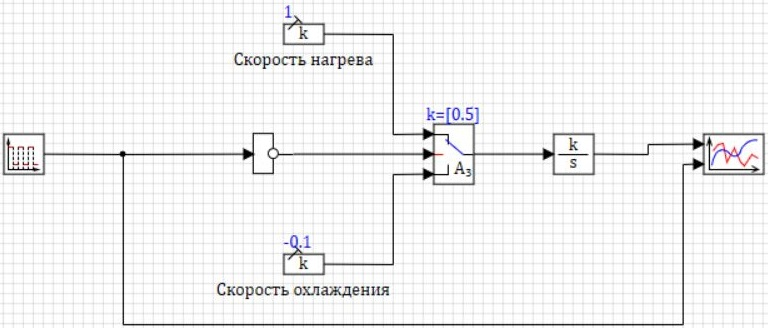
\includegraphics[width=0.8\linewidth]{view_2.JPG}

\center{\caption{Рисунок 1. Схема для проверки модели нагревателя.}}

Результат моделирования показан на рисунке 4. В периоды времени, когда значение меандра равно 1 (имитация включенного нагревателя), модель за счет интегратора накапливает температуру со скоростью нагрева. В периоды, когда значения меандра равны 0 (имитация выключенного нагревателя), температура снижается со скоростью охлаждения.

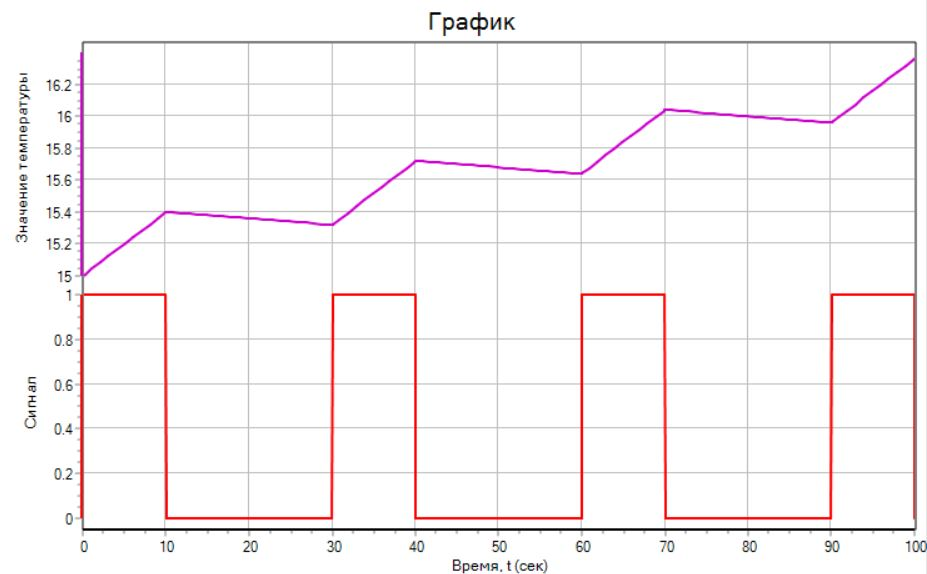
\includegraphics[width=0.75\linewidth]{view_1.JPG}

\caption{Рисунок 2. График работы модели нагревателя.}

Таким образом, мы убедились, что созданная модель может быть
использована для проверки работы контроллера нагревателя.

\section{Создание блока управления нагревателем на базе конечных
автоматов и логики работы состояния}

В нашем случае начальным состоянием автомата будет состояние «выключен». Выделите блок кликом и нажмите правой кнопкой мыши. В выпадающем меню выберите пункт «Свойства». Появится окно редактирования свойств, в котором нужно выбрать «да» в единственном свойстве «По умолчанию».

У блока состояния автомата «включен» два дополнительных порта, блок содержит:
• один входной порт для перехода в состояние (красного цвета);
• один входной порт для данных (черного цвета);
• два выходных порта для перехода из состояния (красного цвета).
Соедините порты, как показано на рисунке 3.

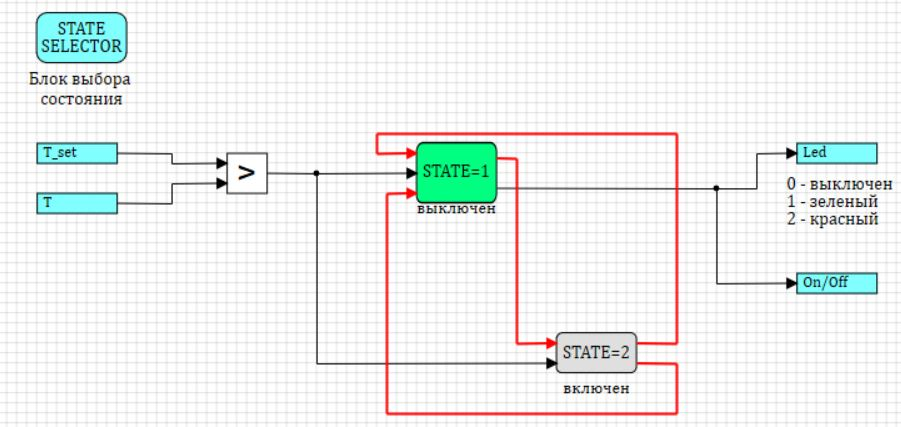
\includegraphics[width=0.75\linewidth]{view_4.JPG}

\caption{Рисунок 3. Логика работы конечного автомата в сборе.}

Таким образом, мы подготовили модель управления на основе конечных автоматов к тестированию. На данном этапе выход на индикатор мы подключили к порту включения, чтобы исключить ошибку, связанную с неподключенным входным портом. 

Результаты моделирования представлены на рисунках 4 (режим работы нагревателя) и 5 (температура Бойлера). На графике режима работы видно, что в начальный момент времени автомат находится в состоянии «выключен» (Рисунок 4)

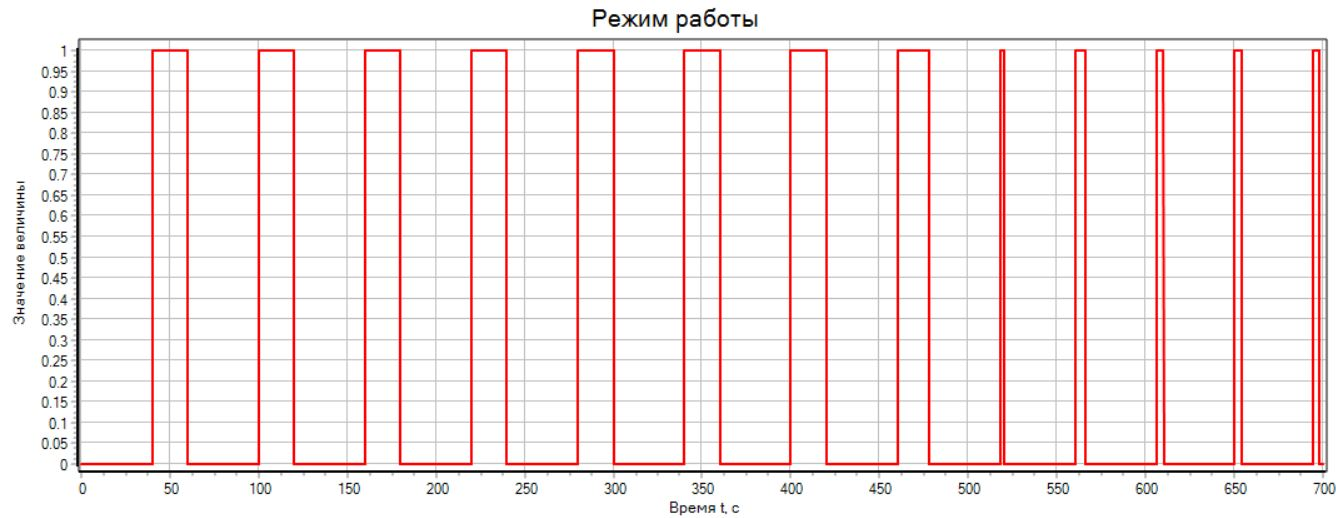
\includegraphics[width=0.9\linewidth]{view_5.JPG}

\caption{Рисунок 4. Режим работы нагревателя.}

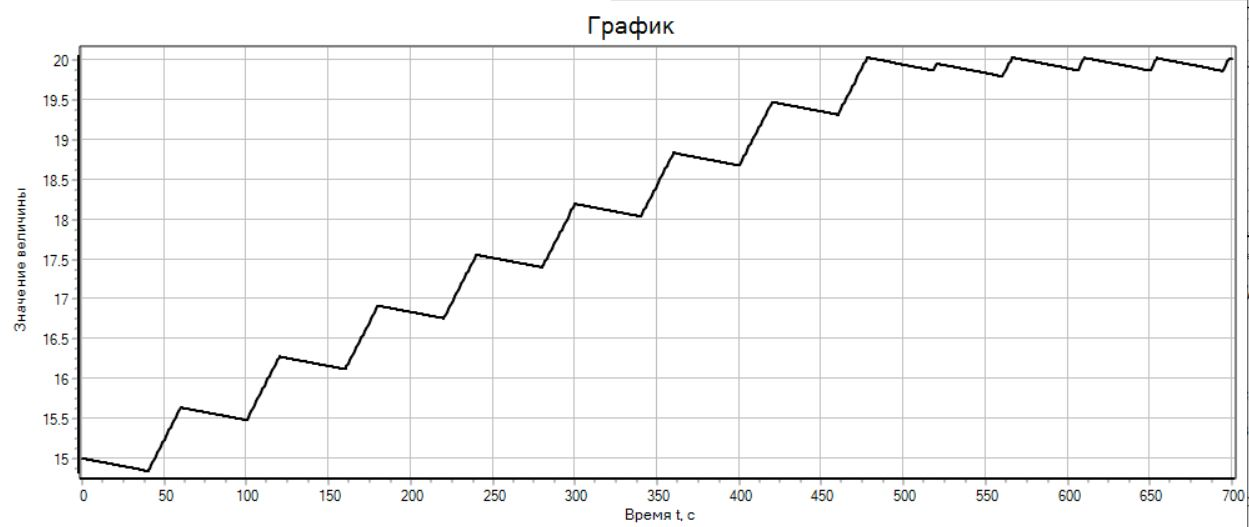
\includegraphics[width=0.9\linewidth]{view_6.JPG}

\caption{Рисунок 5. Температура нагревателя.}

На графике температуры (Рисунок  5) видно, что в начальный момент температура равна 15 градусам и снижается со скоростью охлаждения. После нахождения в состоянии «выключен» в течении 40 секунд происходит переход в состояние «включен» (см. Рисунок  4). В данном состоянии происходит нагрев со скоростью, заданной в модели нагревателя (Рисунок  5). После отработки в течение 10 секунд происходит переход в состояние «выключен» (Рисунок  4). 

Данные циклы повторяются до тех пор, пока температура не достигнет уставки в 20 градусов. После этого цикл включения сокращается, поскольку переход из состояния «включен» в состояние «выключен» осуществляется по достижению уставки по температуре. Это видно на графике «Режим работы» после 500 секунды расчета (Рисунок  4).

Таким образом, мы убедились, что модель управления на базе логики
конечных автоматов работает и поддерживает заданную температуру в
нагревателе.

%http://vv206.veloblog.tk/vv206_files_archive/3%20%D1%81%D0%B5%D0%BC%D0%B5%D1%81%D1%82%D1%80/%D0%A2%D0%B5%D0%BE%D1%80%D0%B8%D1%8F%20%D0%B0%D0%B2%D1%82%D0%BE%D0%BC%D0%B0%D1%82%D0%BE%D0%B2/filelist.html
\end{document}
